\documentclass[../reportesINE.tex]{subfiles}

\begin{document}

\subsection{Perspectiva del módulo}
La dirección jurídica cuenta con 4 sistemas uno por cada área (\textit{Imagen \ref{fig:sistemasDJ}}) y diecisiete subprocesos (\textit{Imagen \ref{fig:subprocesosDJ}}). 
\\ \\
Se solicita el desarrollo de un módulo para la consulta de datos de cada subproceso. Los datos deben encontrarse en todo momento actualizados. Descripción breve del módulo \textit{Imagen \ref{fig:modulo}} 
\\ \\
En relación a los datos y aplicaciones, el sistema deberá proporcionar información precisa, oportuna, completa y ordenada sobre los datos que se generen de las actividades que integran cada uno de los procesos antes listados, en sus tres especificaciones funcionales básicas: entradas, almacenamiento y salidas. Por lo que se deberá implementar gobernabilidad de datos \footnote{Entendiendo por gobernabilidad de datos, como la capacidad de una organización para gestionar el conocimiento que tiene sobre su información. El gobierno de datos proporciona un enfoque holístico para administrar, mejorar y aprovechar la información de forma que pueda ayudarnos a ganar percepción y generar confianza en decisiones y operaciones empresariales.}, para garantizar la entrega de datos fiables y seguros, de acuerdo a las reglas que la Dirección Jurídica establezca.

\begin{figure}[h]
  \centering
  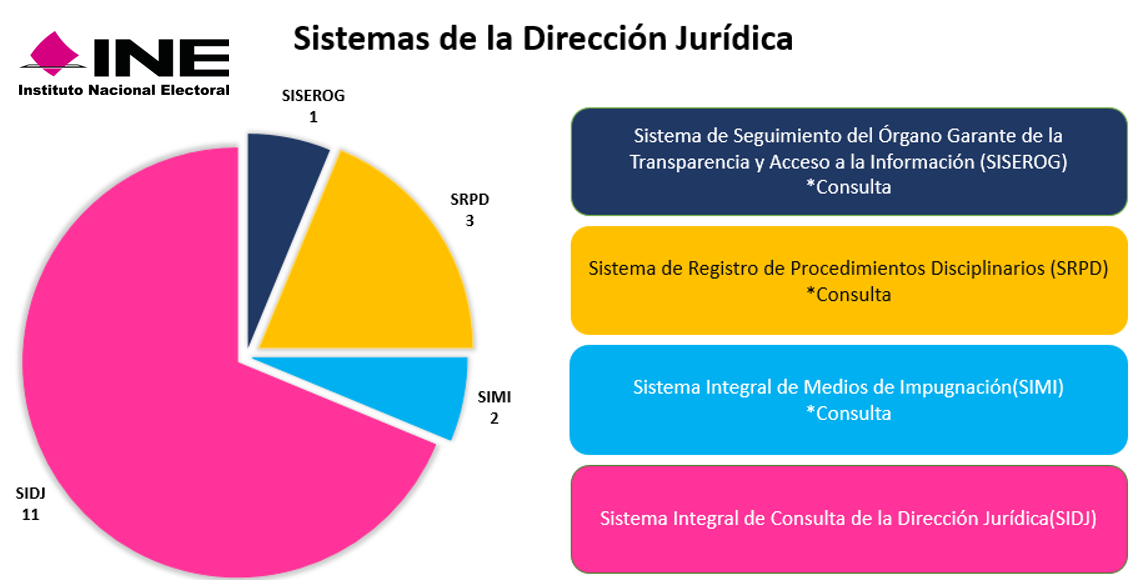
\includegraphics[width=\linewidth]{img/sistemasDJ.PNG}
  \caption{Sistemas de la Dirección jurídica.}
  \label{fig:sistemasDJ}
\end{figure}

\begin{figure}
  \centering
  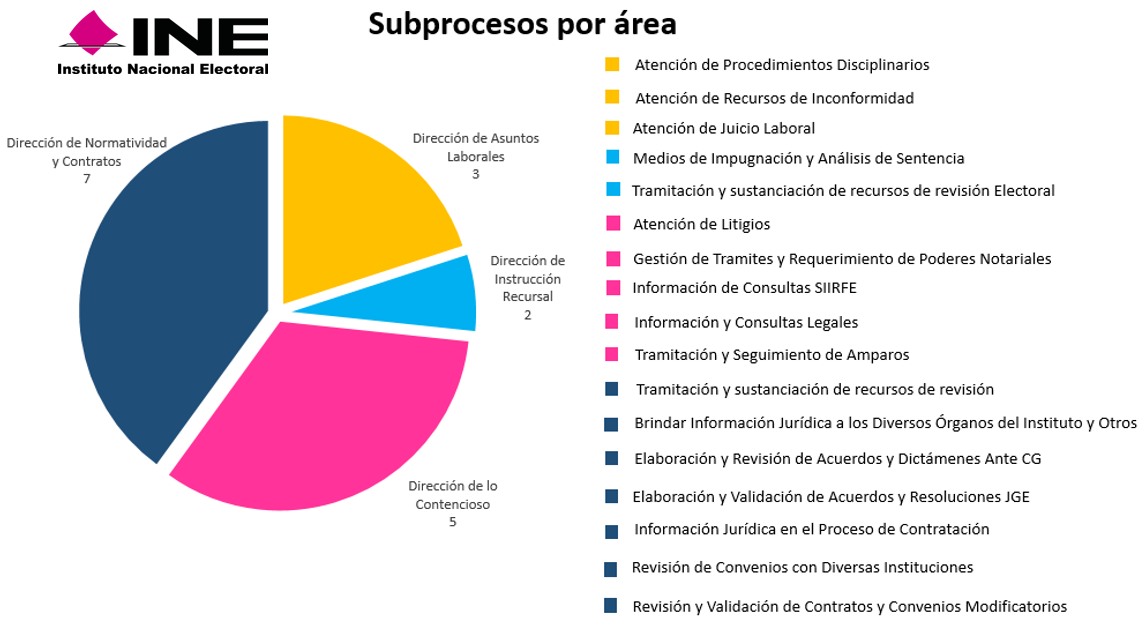
\includegraphics[width=\linewidth]{img/subprocesosDJ.PNG}
  \caption{Subprocesos de la Dirección jurídica.}
  \label{fig:subprocesosDJ}
\end{figure}

\begin{figure}
  \centering
  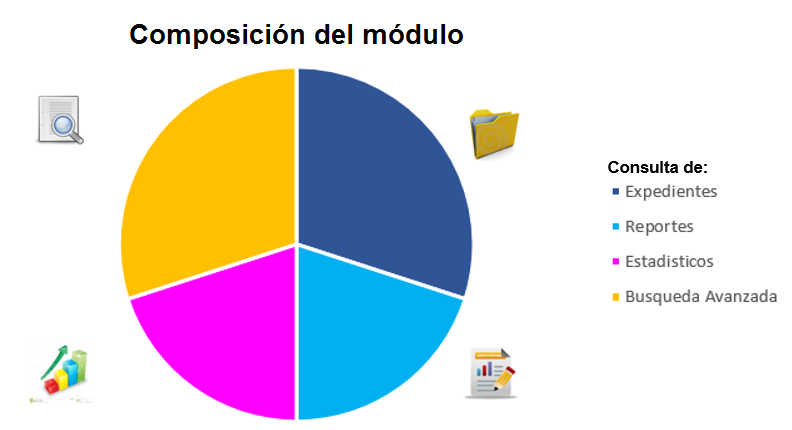
\includegraphics[width=\linewidth]{img/modulo.PNG}
  \caption{Funcionalidad requerida en el módulo de reportes.}
  \label{fig:modulo}
\end{figure}


\subsection{Requerimientos funcionales}
Para los requerimientos no fuincionales tenemos los servicios que debe proporcionar el sistema, de la manera en que éste debe reaccionar a entradas particulares y de cómo se debe comportar en situaciones particulares. En algunos casos, los requerimientos funcionales de los sistemas también pueden declarar explícitamente lo que el sistema no debe hacer. los requerimientos funcionales de un sistema describen lo que el sistema debe hacer. Estos requerimientos dependen del tipo de software que se desarrolle, de los posibles usuarios del software y del enfoque general tomado por la organización al redactar requerimientos. \\ \\
Los requerimientos funcionales para un sistema software se pueden expresar de diferentes formas. a continuación se presentan dichos requerimientos para el módulo de consulta del \textit{Sistema Integral de la Dirección Jurídica}. \\

\begin{itemize}
\item Integrar consulta de información de cada uno de los procesos especificados en la \textit{Dirección Jurídica}. \\
\item Ser construido sobre un concepto de autómatas inteligentes, capaz de establecer una tramitación guiada al usuario, de manera intuitiva y simple dentro de la aplicación proponiendo opciones de acuerdo a los diferentes factores que especifique el proceso. \\
\item Integrar esquema de control de acceso para la identificación, autenticación y autorización de los usuarios a la consulta de datos disponibles en el sistema. \\
\item Funcionalidad para el manejo de datos sensibles. \\
\item Deberá incluir la funcionalidad para obtener informes y reportes de indicadores, estadísticas que faciliten acciones proactivas. 
\item Integrar consultas de información actualizada, tanto para su publicación como para la toma de decisiones. \\
\item Interoperabilidad con otros sistemas del Instituto que provean información al \textit{Sistema Integral de la Dirección Jurídica}. \\
\item Funcionalidad para la exportación de información a formatos como Excel o PDF. \\
\item Implementar mecanismos para garantizar la integridad, confiabilidad y disponibilidad de la información que integre al SIDJ.
\end{itemize}

\subsection{Requerimientos no funcionales}
Son restricciones de los servicios o funciones ofrecidos por el sistema. incluyen restricciones de tiempo, sobre el proceso de desarrollo y estándares. los requerimientos no funcionales a menudo se aplican al sistema en su totalidad. normalmente apenas se aplican a características o servicios individuales del sistema.  \\ \\
Los requerimientos no funcionales, como su nombre sugiere, son aquellos requerimientos que no se refieren directamente a las funciones específicas que proporciona el sistema, sino a las propiedades emergentes de éste como la fiabilidad, el tiempo de respuesta y la capacidad de almacenamiento. De forma alternativa, definen las restricciones del sistema como la capacidad de los dispositivos de entrada/salida y las representaciones de datos que se utilizan en las interfaces del sistema. 

\begin{itemize}
\item Integridad de información entre los sistemas. \\
\item Integridad del esquema de sincronización. \\
\item Capacidad del sistema de trabajar en cualquier computadora con conexión a internet. \\
\end{itemize}

\subsection{Usabilidad}
La Usabilidad es la medida de la calidad de la experiencia que tiene un usuario cuando interactúa con un producto o sistema. Esto se mide a través del estudio de la relación que se produce entre las herramientas (entendidas en un Sitio Web el conjunto integrado por el sistema de navegación, las funcionalidades y los contenidos ofrecidos) y quienes las utilizan, para determinar la eficiencia en el uso de los diferentes elementos ofrecidos en las pantallas y la efectividad en el cumplimiento de las tareas que se pueden llevar a cabo a través de ellas. \\ \\
La interacción entre el módulo y el usuario será, a través del \textit{Sistema Integral de la Dirección Jurídica} platforma web.  \\ \\
La interfaz de la aplicación debe ser amigable y de fácil entendimiento para el usuario, permitiendole realizar sus tareas de forma fácil y sencilla. Procurando siempre que el módulo sea de ayuda para el usuario y no un óbstaculo.

\subsection{Confiabilidad}
Un software supuesto para ser utilizado solamente por aquellos autorizados, debe procurar detectar y excluir el desautorizado. El acceso a él por lo tanto es controlado generalmente insistiendo en un procedimiento de la autentificación para establecer con un cierto grado establecido de confianza la identidad del usuario, por lo tanto concediendo esos privilegios como puede ser autorizado a esa identidad. \\ \\
El control de acceso al módulo será controlado por una validación de nombre de usuario y contraseña.  \\ \\
De esta manera para que un usuario pueda ingresar al módulo debe haber sido previamente autorizado por el administrador de la aplicación, quien creará un nombre de usuario y una contraseña asociado a un perfil tipo consulta, el cual tendrá los permisos y funcionalidades necesarios para la consulta de datos y generación de reportes.


\end{document}